\documentclass[conference]{IEEEtran}
\IEEEoverridecommandlockouts
% ---------------------------------------------------------------------------
% Packages
% ---------------------------------------------------------------------------
\usepackage{cite}
\usepackage{amsmath,amssymb,amsfonts}
\usepackage{graphicx}
\usepackage{textcomp}
\usepackage{xcolor}
\usepackage{booktabs}
\usepackage{url}
\usepackage{tikz}
\usetikzlibrary{positioning,arrows.meta,calc}
\def\BibTeX{{\rm B\kern-.05em{\sc i\kern-.025em b}\kern-.08em
    T\kern-.1667em\lower.7ex\hbox{E}\kern-.125emX}}

\begin{document}

\title{Molly: A Lightweight C++ Game Engine \\ with an Integrated Level Editor\thanks{Identify applicable funding agency here. If none, delete this.}}

% ---------------------------------------------------------------------------
% Author block
% ---------------------------------------------------------------------------
\author{
\IEEEauthorblockN{Maharun Afroz}
\IEEEauthorblockA{
\textit{Dept. of Electrical and Computer Engineering} \\
\textit{North South University} \\
Dhaka, Bangladesh \\
maharun.afroz@northsouth.edu}
\and
\IEEEauthorblockN{Nasif Atique Chowdhury}
\IEEEauthorblockA{
\textit{Dept. of Electrical and Computer Engineering} \\
\textit{North South University} \\
Dhaka, Bangladesh \\
nasif.chowdhury01@northsouth.edu}
\and
\IEEEauthorblockN{Dr. Shahnewaz Siddique}
\IEEEauthorblockA{
\textit{Dept. of Electrical and Computer Engineering} \\
\textit{North South University} \\
Dhaka, Bangladesh \\
shahnewaz.siddique@northsouth.edu}
}

\maketitle

\begin{abstract}
Commercial game engines such as Unity, Unreal Engine, and Godot provide
powerful tooling, but their scale and partially closed architectures make
them difficult vehicles for understanding how a game engine actually
works internally. This paper presents Molly, a lightweight, from-scratch
3D game engine written in modern C++20 for Windows, built as the first
half (CSE499A) of a two-part junior design project. Molly combines a
forward OpenGL 4.6 renderer, an entity-component-system (ECS) built on
\texttt{entt}, the Jolt physics engine, Lua scripting via
\texttt{sol2}, and a Dear ImGui-based visual editor, with every
third-party dependency vendored directly inside the project repository.
The engine was validated end-to-end with a playable demonstration game
and an automated test suite. This paper describes the system
architecture, the editor tooling built on top of the engine, notable
engineering challenges encountered during development, a quantitative
characterization of the resulting codebase and test suite, and a
structured audit of the engine's current limitations, which defines the
proposed scope of CSE499B.
\end{abstract}

\begin{IEEEkeywords}
Game Engine, Entity-Component-System, OpenGL, Real-Time Rendering,
Physics Simulation, Scripting, Level Editor
\end{IEEEkeywords}

% =============================================================================
\section{Introduction and Problem Statement}
% =============================================================================

Real-time 3D applications -- games in particular -- are built on top of
game engines: reusable software frameworks that provide rendering,
physics simulation, audio, input, and content-authoring tools so that
game-specific logic does not need to be built from raw graphics and
platform APIs each time. Commercial engines such as Unity, Unreal
Engine, and Godot are the dominant choice in industry, but their scale
and, in the case of Unity and Unreal, partially closed-source
architecture make them difficult to use as a learning vehicle for
understanding how an engine's subsystems are actually wired together --
how a renderer, a physics simulation, a scripting layer, and a visual
editor combine into a single coherent application.

\subsection{Problem Statement}
\label{sec:problem}

Existing avenues for learning game engine internals are each
insufficient on their own. Reading commercial engine source where it is
available (e.g. Unreal Engine) means navigating a codebase of millions
of lines built for production concerns -- platform abstraction,
backward compatibility, plugin systems -- that obscure rather than
illustrate the core architecture. Small ``build your own engine''
tutorials, at the other extreme, typically stop at a renderer or a
minimal ECS and never integrate physics, scripting, serialization, and
an editor into one coherent, working application, so the reader never
sees how these subsystems' design decisions constrain each other in
practice (e.g. how the editor's Play-mode scene cloning interacts with
physics-world lifetime, discussed in Section~\ref{sec:related}). The
problem this project addresses is therefore: \emph{build a game engine
small enough to be understood end-to-end by its own developers, yet
complete enough -- rendering, ECS, physics, scripting, resource
management, serialization, audio, and a visual editor -- to validate
that its subsystems genuinely integrate, rather than existing as
isolated demonstrations.}

Molly was built to close that gap: a minimal but functionally complete
engine, small enough to be understood in full, but structured the way a
real engine is structured, with a clean separation between a reusable
engine library, an editor application, and a sample game that consumes
the engine through the same public API a third-party game would use.

The objectives set for CSE499A were to: (1) build a working real-time 3D
rendering pipeline using OpenGL 4.6; (2) integrate an
entity-component-system as the engine's core data model; (3) add
rigid-body physics simulation and collision detection; (4) support
gameplay scripting through an embedded language, decoupling gameplay
logic from engine C++ code; (5) build a resource/asset management layer
with hot-reloading; (6) build a visual, ImGui-based level editor
comparable in layout and workflow to industry-standard tools; (7)
support saving and loading of scenes and prefabs as human-readable data;
(8) add positional 3D audio; and (9) validate the engine end-to-end with
a small playable demonstration game.

% =============================================================================
\section{Related Work}
\label{sec:related}
% =============================================================================

Two broad philosophies exist for how gameplay logic is authored in a
game engine. \textbf{Data-driven} engines -- Unity, Godot, Unreal --
have scenes, prefabs, and scripts authored entirely inside a visual
editor, with a generic, pre-compiled runtime loading and executing that
data, so that shipping a new game does not require recompiling the
engine itself. \textbf{Code-first} engines -- id Tech, Source, and other
Quake-era engines -- instead compile gameplay logic as C/C++ code linked
directly against the engine as a library, with the editor serving
primarily as a level/content-authoring tool feeding a separately
compiled game binary. Molly currently sits between the two: it supports
data-driven scenes and prefabs (serialized to JSON) and Lua-scripted
gameplay logic, but does not yet have a generic runtime capable of
shipping a game without an accompanying hand-written C++ project, which
Section~\ref{sec:limitations} discusses as a direction for CSE499B.

The engine's core data model follows the entity-component-system (ECS)
pattern, which separates \emph{identity} (an entity, an integer handle),
\emph{data} (components -- plain structs with no behaviour), and
\emph{behaviour} (systems -- functions operating over sets of
components) \cite{gregory-gea,nystrom-gpp}. Nystrom \cite{nystrom-gpp}
frames this as a deliberate rejection of deep inheritance hierarchies in
favour of composition, motivated by the same problem West's earlier,
widely cited industry article identifies: object-oriented inheritance
trees in game entities tend to force awkward multiple-inheritance or
god-object designs once an entity needs behaviour that cuts across
unrelated branches of the hierarchy (e.g. something that is simultaneously
damageable, renderable, and physically simulated) \cite{west-evolve}.
An entity in this pattern is not a class in an inheritance hierarchy but
simply a handle that happens to carry a transform component, a mesh
renderer component, a rigid body component, and a script component.
Molly uses \texttt{entt} \cite{entt}, a widely used header-only,
sparse-set-based ECS library, for this layer.

Molly's forward-rendering pipeline and Blinn-Phong-style lighting model
follow standard real-time rendering practice as described by
Akenine-M{\"o}ller et al. \cite{rtr4}, targeting the OpenGL 4.6 core
profile as specified by the Khronos Group \cite{opengl46}. Its rigid-body
physics layer (Jolt \cite{jolt}) implements the discrete, iterative
constraint-solving approach common to real-time game physics engines, as
described by Millington \cite{millington-physics}, rather than the
continuous, offline-tolerant methods used in engineering simulation
software.

% =============================================================================
\section{System Architecture}
% =============================================================================

Molly is organized as a CMake multi-target project with three build
targets, all self-contained inside the repository: every third-party
dependency is vendored as a git submodule under \texttt{vendor/}, with
no reliance on an external package manager such as vcpkg or Conan.
\texttt{molly-engine} is a static library containing every reusable
subsystem (application loop, renderer, ECS, physics, scripting, resource
management, audio, scene serialization). \texttt{molly-editor} is the
visual editor application, linking \texttt{molly-engine} and adding
editor-only panels and tooling. \texttt{molly-demo} is a hand-written
sample game linking \texttt{molly-engine} directly, used both as a
demonstration and as an integration test of the engine's public API
surface.

Figure~\ref{fig:architecture} illustrates this layering: the editor and
demo game are independent executables that both link the same engine
library, which in turn is built on top of the vendored third-party
libraries listed in Table~\ref{tab:vendor}.

\begin{figure}[htbp]
\centering
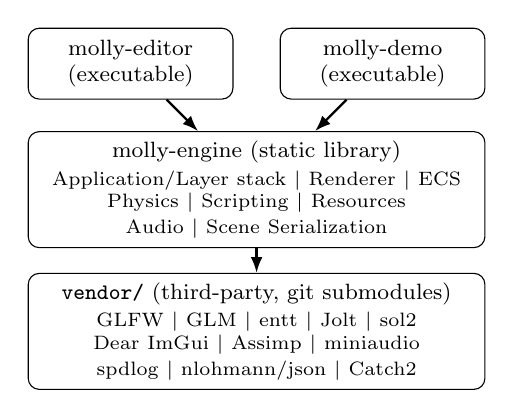
\begin{tikzpicture}[
    box/.style={draw, rounded corners, align=center, minimum height=0.9cm, font=\footnotesize},
    arrow/.style={-{Latex[length=2mm]}, thick}
]
\node[box, minimum width=2.6cm] (editor) at (0,3) {molly-editor \\ (executable)};
\node[box, minimum width=2.6cm] (demo) at (3.2,3) {molly-demo \\ (executable)};
\node[box, minimum width=5.8cm, text width=5.4cm] (engine) at (1.6,1.4)
    {molly-engine (static library) \\[2pt]
     \scriptsize Application/Layer stack \textbar\ Renderer \textbar\ ECS \\
     \scriptsize Physics \textbar\ Scripting \textbar\ Resources \\
     \scriptsize Audio \textbar\ Scene Serialization};
\node[box, minimum width=5.8cm, text width=5.4cm] (vendor) at (1.6,-0.4)
    {\texttt{vendor/} (third-party, git submodules) \\[2pt]
     \scriptsize GLFW \textbar\ GLM \textbar\ entt \textbar\ Jolt \textbar\ sol2 \\
     \scriptsize Dear ImGui \textbar\ Assimp \textbar\ miniaudio \\
     \scriptsize spdlog \textbar\ nlohmann/json \textbar\ Catch2};
\draw[arrow] (editor) -- (engine);
\draw[arrow] (demo) -- (engine);
\draw[arrow] (engine) -- (vendor);
\end{tikzpicture}
\caption{Molly's build-target layering: independent executables linking
a shared engine static library, itself built on vendored third-party
dependencies.}
\label{fig:architecture}
\end{figure}

Table~\ref{tab:vendor} lists the third-party libraries vendored inside
the repository and their purpose.

\begin{table}[htbp]
\caption{Third-party libraries vendored inside the repository}
\label{tab:vendor}
\centering
\begin{tabular}{ll}
\toprule
\textbf{Library} & \textbf{Purpose} \\
\midrule
GLFW \cite{glfw} & Window creation, input, GL context \\
GLAD & OpenGL 4.6 function loader \\
GLM & Vector/matrix math \\
entt \cite{entt} & Entity-component-system \\
Jolt Physics \cite{jolt} & Rigid-body physics, collision \\
Lua + sol2 \cite{sol2} & Scripting and its C++ binding layer \\
Dear ImGui \cite{imgui} & Immediate-mode GUI (editor) \\
Assimp & 3D model import (glTF, OBJ, FBX) \\
stb\_image & Texture decoding (PNG/JPG) \\
miniaudio & Cross-platform audio playback \\
spdlog & Structured logging \\
nlohmann/json & Scene/prefab serialization \\
Catch2 & Unit/integration testing \\
\bottomrule
\end{tabular}
\end{table}

The engine follows a layer-stack architecture. An \texttt{Application}
owns a \texttt{Window}, a \texttt{ResourceManager}, an
\texttt{AudioEngine}, and a stack of \texttt{Layer} objects. Each frame:
every layer's \texttt{onUpdate(dt)} runs (game logic, physics stepping,
camera movement); an ImGui frame begins; every layer's
\texttt{onImGuiRender()} runs (UI panels, the 3D viewport); the ImGui
draw data is rendered; and the window swaps buffers and polls OS events.
This ordering -- update before the ImGui frame begins, event polling
after everything is presented -- has a subtle consequence discussed in
Section~\ref{sec:challenges}.

\subsection{Comparison with Existing Engines}
\label{sec:comparison}

Table~\ref{tab:comparison} positions Molly against the three commercial
engines discussed in Section~\ref{sec:related}, across axes relevant to
this project's stated problem (Section~\ref{sec:problem}): source
availability, scripting approach, and dependency self-containment,
rather than production-readiness metrics where a two-target-executable
student project cannot meaningfully compete with engines developed by
hundreds of engineers over a decade or more.

\begin{table}[htbp]
\caption{Molly vs.\ established engines, by architectural transparency}
\label{tab:comparison}
\centering
\footnotesize
\begin{tabular}{lp{1.5cm}p{1.5cm}p{1.5cm}p{1.5cm}}
\toprule
& \textbf{Molly} & \textbf{Unity} & \textbf{Unreal} & \textbf{Godot} \\
\midrule
Engine source available & Yes, full & No (core closed) & Yes, full & Yes, full \\
Scripting language & Lua & C\# & C++/ Blueprints & GDScript/C\# \\
Dependencies & Vendored, no package mgr. & Closed, bundled & Vendored + Perforce & Vendored \\
Editor included & Yes & Yes & Yes & Yes \\
Primary design goal & Educational transparency & Production, broad platform reach & Production, AAA fidelity & Production, open-source community \\
\bottomrule
\end{tabular}
\end{table}

The comparison's purpose is not to claim feature parity -- Molly has no
shadows, no PBR materials, and no shipping pipeline
(Section~\ref{sec:limitations}) -- but to make explicit what Molly
optimizes for that the others do not: every line between a keystroke in
the editor and a pixel on screen is first-party code the project's own
developers wrote and can read, which is precisely the property the
problem statement (Section~\ref{sec:problem}) identifies as missing from
existing learning resources.

\subsection{Design Requirements and Constraints}
\label{sec:requirements}

The following non-functional requirements were set at project outset and
constrained every subsequent design decision:

\begin{itemize}
    \item \textbf{Self-containment.} No external package manager
          (e.g. vcpkg, Conan) may be used; every third-party dependency
          is vendored as a git submodule inside the repository, so the
          project builds from a single \texttt{git clone} plus CMake,
          with no separate dependency-installation step.
    \item \textbf{Platform scope.} Windows 10/11 only, targeting OpenGL
          4.6 core profile on hardware supporting it. Cross-platform
          support is explicitly out of scope for CSE499A (Table~\ref{tab:gaps}).
    \item \textbf{Human-readable persistence.} Scenes and prefabs must
          serialize to plain-text JSON rather than a binary format, so
          they can be diffed and version-controlled meaningfully.
    \item \textbf{Real-time responsiveness.} The editor and any game
          built on the engine must sustain interactive frame rates
          (target: 60\,FPS) under typical editing/gameplay loads on
          consumer hardware.
    \item \textbf{Fault containment.} A single malformed script or
          missing asset must degrade gracefully (a logged error, an
          unloaded/placeholder resource) rather than crash the entire
          application -- verified in practice for both cases in
          Section~\ref{sec:testing}.
\end{itemize}

\subsection{Software Engineering Methodology and Design Patterns}
\label{sec:se}

Consistent with software engineering practice covered in CSE327, Molly
was developed under an \textbf{incremental development model} rather
than a waterfall or big-bang approach: the requirements in
Section~\ref{sec:requirements} were fixed up front, but implementation
proceeded as a sequence of independently buildable, independently
testable increments (renderer, then ECS, then physics, then scripting,
and so on), each of which left both executables in a working,
demonstrable state before the next increment began. This is a
risk-reduction strategy in the classical sense: a defect introduced in
one increment (Section~\ref{sec:challenges}) is far cheaper to localize
and fix when only that increment's code has changed since the last known-good
state, than it would be to debug after all subsystems were written
simultaneously.

Several standard design patterns and software engineering principles
are used deliberately, not incidentally:

\begin{itemize}
    \item \textbf{Layered architecture.} \texttt{molly-engine} exposes a
          public API consumed identically by \texttt{molly-editor} and
          \texttt{molly-demo} (Figure~\ref{fig:architecture}); neither
          consumer depends on the other, and the engine layer depends on
          neither, enforcing a strict, testable dependency direction.
    \item \textbf{Composition over inheritance (ECS).} As discussed in
          Section~\ref{sec:related}, entity behaviour is composed from
          independent components rather than derived through an
          inheritance hierarchy, directly avoiding the fragile-base-class
          and diamond-inheritance problems that hierarchy-based entity
          designs are documented to suffer from \cite{west-evolve}.
    \item \textbf{Observer pattern (event dispatch).} Window/input
          events are dispatched top-down through the layer stack via an
          \texttt{EventDispatcher}, decoupling event \emph{producers}
          (GLFW callbacks) from event \emph{consumers} (individual
          layers), each of which may mark an event handled and stop
          propagation.
    \item \textbf{Facade pattern.} \texttt{Application} presents a
          single, simplified interface (\texttt{run()},
          \texttt{pushLayer()}, \texttt{getWindow()}, ...) over several
          independently complex subsystems (windowing, resource
          management, audio, ImGui), so a consumer never needs to
          understand or directly wire together their internal
          interactions.
    \item \textbf{Separation of concerns (Model-View).} A \texttt{Scene}
          and its entities are pure data with no rendering or UI
          knowledge; the editor's panels (Hierarchy, Inspector, Viewport)
          are a separate, replaceable presentation layer over that same
          data, and the same \texttt{Scene} is consumed with zero
          modification by the non-visual \texttt{molly-demo} game.
    \item \textbf{Verification and validation.} Automated unit/integration
          testing (Catch2, Section~\ref{sec:testing}) validates
          component-level correctness; manual/structural verification
          (log inspection, \texttt{imgui.ini} structure checks) validates
          behaviour the automated suite does not yet reach -- an
          explicit, acknowledged gap (Section~\ref{sec:limitations})
          rather than an oversight.
    \item \textbf{Version control discipline.} The project uses a
          single-trunk git workflow with all third-party code isolated
          under \texttt{vendor/} as pinned submodules, keeping first-party
          history (Table~\ref{tab:results}) cleanly separated from
          dependency history.
\end{itemize}

% =============================================================================
\section{The Editor}
\label{sec:editor}
% =============================================================================

The first version of the editor's docking layout relied solely on
ImGui's viewport-spanning dockspace helper, which creates a dockspace
\emph{host} but does not itself assign any panel to a dock node. In
practice, every panel fell back to ImGui's default cascading window
placement, producing an overlapping, unusable layout. The fix uses
ImGui's internal dock-builder API to explicitly construct a Unity/Godot-style
default arrangement the first time the editor runs: Hierarchy docked
left, Inspector docked right, Content Browser and Console tabbed
together along the bottom, and the Viewport occupying the remaining
central space. This was verified both visually and structurally, by
inspecting the auto-generated \texttt{imgui.ini} layout file to confirm
the dock-node sizes and identifiers matched the intended layout.

A pinned toolbar (Play/Pause/Stop transport controls and a color-coded
play-state badge) and status bar (status messages, active scene name,
selection count, play state, frame rate) were added outside the
dockspace. The main menu bar provides File, Window (layout reset and
per-panel visibility toggles), Edit, and Help menus. A consistent accent
color theme replaces ImGui's stock dark theme, applied once in the
shared ImGui layer so both the editor and the demo game's debug UI
inherit it.

Beyond displaying the rendered scene, the viewport implements a
free-fly editor camera, scroll-wheel dolly zoom, a ``frame selected''
shortcut matching the Unity/Unreal/Blender convention, a wireframe
selection outline drawn over the selected entity, and wireframe gizmo
markers for light and camera entities, which render no mesh of their
own and would otherwise be impossible to locate or select in the 3D
view.

% =============================================================================
\section{Engineering Challenges}
\label{sec:challenges}
% =============================================================================

Several defects encountered during development were significant enough,
in both symptom and root cause, to document explicitly.

\subsection{Missing Depth Testing}
After the editor UI overhaul, only the scene's floor plane was visible
in the viewport; a box prop placed at the origin rendered as nothing.
The cause was that depth testing was never enabled anywhere in the
engine. Without it, fragments are written to the framebuffer in whatever
order the ECS iterates entities -- and \texttt{entt} iterates its
component pools in reverse creation order -- rather than by distance to
the camera. The floor plane, created after the prop, was drawn
\emph{on top of} the prop and overwrote it despite being farther from
the camera. The fix was enabling depth testing with a standard
less-than comparison in the engine's shared render entry point.

\subsection{Mouse-Wheel Input Timing}
Scroll-wheel zoom, when first implemented, silently did nothing. The
cause was a mismatch between the engine's frame-loop ordering and Dear
ImGui's input-event model: scroll deltas are queued by the windowing
callback and only merged into ImGui's per-frame mouse-wheel state inside
its new-frame call. The zoom logic had been placed in the viewport
panel's per-frame update function, which the application loop runs
\emph{before} that new-frame call, so it was always reading a stale
value. Moving the read to the panel's ImGui-render function, alongside
the existing hover-detection code that already ran in the correct order,
resolved the issue.

\subsection{Working-Directory Dependence}
Every relative asset path in the engine (shaders, textures, models, log
files, the editor's window icon) was resolved against the process's
current working directory. This worked when the editor was launched
from a terminal already positioned in its source directory, but failed
silently when launched by double-clicking the executable, since that
lands in the build output directory, which never had assets copied into
it. The fix changes the process's working directory to the executable's
own directory as the first statement in \texttt{main()}, paired with a
CMake post-build step that copies each target's assets folder next to
its built executable.

\subsection{Invisible Selection for Non-Mesh Entities}
The ``frame selected'' feature appeared broken for light and camera
entities specifically, while working correctly for mesh-bearing
entities. The camera was, in fact, moving to the correct position in
both cases -- but light and camera entities have no mesh to render, so
framing them centered the view on nothing visible. This was resolved by
adding wireframe gizmo markers (Section~\ref{sec:editor}), giving every
entity type a visible representation regardless of whether it owns a
mesh.

\subsection{Discussion}

Three of the four defects above -- missing depth testing, the
mouse-wheel timing bug, and the invisible-selection issue -- share a
common root cause pattern: an \emph{implicit ordering or existence
assumption} that held in the simple case first tested but broke under a
slightly different, equally valid input. Depth testing was never needed
while the scene contained only one visible object; frame ordering only
mattered once a feature (scroll input) depended on exactly which side of
\texttt{NewFrame()} it ran on; and selection-framing only broke for
entity types (lights, cameras) that were never the ones used while
building and testing the feature. This suggests a general lesson for the
engine's continued development: features should be exercised against a
scene deliberately constructed to violate the assumption most likely to
be silently relied upon (multiple overlapping objects, non-default input
timing, entities without the "expected" component set), rather than
against whatever scene happens to already be open.

% =============================================================================
\section{Testing}
\label{sec:testing}
% =============================================================================

Correctness was validated at two levels. A Catch2-based automated test
suite exercises the engine's serialization round-trips (scene and prefab
save/load producing an equivalent entity graph) and core component
behaviour (transform, physics, light, camera, and script components);
at the end of CSE499A the suite comprises 45 assertions across 7 test
cases, all passing. This suite does \emph{not} cover rendering output
correctness, physics simulation accuracy, or editor UI behaviour --
all three currently rely on the manual/structural verification described
below, and are identified as an automated-coverage gap in
Section~\ref{sec:limitations}.

Because visual correctness cannot be captured by unit tests alone,
editor changes were additionally verified by running the built
executables headlessly and checking log output for load/compile errors,
and by inspecting the auto-generated ImGui layout file directly to
confirm dock-node structure independent of the ability to visually
render the UI. Fault-containment behaviour (Section~\ref{sec:requirements})
was verified directly: a deliberately malformed Lua script produces a
logged error without crashing the application, and a missing texture
path produces a logged error and an unloaded/blank texture rather than a
thrown exception.

% =============================================================================
\section{Results}
\label{sec:results}
% =============================================================================

Table~\ref{tab:results} reports measured characteristics of the codebase
and build artifacts at the end of CSE499A. Line counts exclude all
vendored third-party code under \texttt{vendor/}, counting only
first-party engine, editor, and demo game sources. Executable sizes are
from unoptimized Debug builds (MSVC, \texttt{/Od}, full debug symbols)
on Windows 11 and are reported to characterize build output, not as a
measure of shipping footprint, which would require a Release
configuration. The full automated test suite (45 assertions, 7 test
cases) completes in under 0.3\,s on the development machine (Intel-class
laptop, NVIDIA GeForce RTX 4050 Laptop GPU), confirming the suite is
cheap enough to run on every build rather than being reserved for
periodic checks.

\begin{table}[htbp]
\caption{Measured codebase and runtime characteristics}
\label{tab:results}
\centering
\begin{tabular}{lr}
\toprule
\textbf{Metric} & \textbf{Value} \\
\midrule
Engine source (files / lines) & 74 / 4{,}577 \\
Editor source (files / lines) & 15 / 1{,}481 \\
Demo game source (files / lines) & 3 / 259 \\
Test suite source (lines) & 226 \\
Test suite (assertions / cases) & 45 / 7 \\
Test suite execution time & $<$0.3\,s \\
\texttt{molly-editor.exe} size (Debug) & 18.5\,MB \\
\texttt{molly-demo.exe} size (Debug) & 18.3\,MB \\
\bottomrule
\end{tabular}
\end{table}

As an informal indicator of runtime performance -- not a rigorous
benchmark, since no automated frame-time profiling harness exists yet
(Section~\ref{sec:limitations}) -- the editor sustains approximately
75 frames per second in its default scene (one directional light, a
handful of mesh entities, editor UI overlay) on the development
hardware. A dedicated performance-benchmarking harness, measuring frame
time under increasing entity/light counts, is proposed as part of
CSE499B (Section~\ref{sec:limitations}).

% =============================================================================
\section{Limitations and What Will Be Completed in CSE499B}
\label{sec:limitations}
% =============================================================================

\subsection{Current Limitations}
\label{sec:current-limitations}

A structured audit of the engine's current state was carried out at the
end of CSE499A, distinguishing what exists from what a comparable
production tool would additionally provide. Table~\ref{tab:gaps}
summarizes the findings.

\begin{table}[htbp]
\caption{Engine capabilities vs. known gaps, end of CSE499A}
\label{tab:gaps}
\centering
\footnotesize
\begin{tabular}{p{1.6cm}p{2.9cm}p{2.9cm}}
\toprule
\textbf{Area} & \textbf{What exists} & \textbf{What is missing} \\
\midrule
Rendering & Forward renderer, Blinn-Phong lighting & Shadows, PBR, skybox/IBL, post-processing \\
Viewport & Fly camera, zoom, selection outline, gizmos & Translate/rotate/scale manipulator \\
Scene workflow & Hierarchy/Inspector, scene + prefab JSON & Undo/Redo, multi-select, drag-and-drop \\
Physics & Jolt rigid bodies, colliders, controller & Joint editing, physics debug-draw \\
Shipping & Hand-written \texttt{game/} C++ project & Generic runtime + editor Build/Export \\
Materials & In-memory, per-entity & Standalone, reusable material assets \\
Scene mgmt. & One scene for app lifetime & Runtime level loading/switching \\
Project & Hardcoded relative asset paths & Project file, settings, picker \\
Input & Direct calls per call-site & Centralized input abstraction \\
Script editing & External editor only & In-editor code editor \\
\bottomrule
\end{tabular}
\end{table}

\subsection{What Will Be Completed in CSE499B}
\label{sec:next}

Based on this audit, four items are proposed as priorities for CSE499B:
(1) materials as standalone, reusable assets, so a material can be
authored once and shared across multiple objects rather than inlined per
entity; (2) runtime scene/level switching, so a game built in Molly can
consist of more than a single, permanently loaded scene; (3) a generic
runtime ``player'' and build/export pipeline, removing the need to
hand-write a bespoke C++ project to ship a game; and (4) a viewport
translate/rotate/scale manipulator gizmo, replacing purely numeric
transform editing with direct on-screen manipulation.

A fifth, cross-cutting gap not captured by Table~\ref{tab:gaps} is
automated test coverage itself: as noted in Section~\ref{sec:testing},
the current suite validates serialization and component logic but not
rendering output, physics simulation accuracy, or editor UI behaviour.
Closing this gap -- e.g. golden-image rendering tests, deterministic
physics-replay tests -- is proposed as ongoing work throughout CSE499B
rather than a single milestone.

% =============================================================================
\section{Ethical and Societal Considerations}
% =============================================================================

As a development tool rather than an end-user application, Molly's
direct ethical footprint is limited, but several considerations were
part of its design from the outset. All vendored third-party libraries
(Table~\ref{tab:vendor}) are used under their respective permissive
open-source licenses (MIT, zlib, Apache-2.0, or similar), and Molly
itself is intended for open, unrestricted use and modification,
consistent with its goal as an educational reference implementation. The
engine collects, stores, and transmits no user data of any kind -- it is
an entirely offline, local tool with no network or telemetry code path
-- so it raises no privacy concerns of its own. Its energy footprint is
that of any real-time 3D application (continuous GPU utilization while
running); no specific power-efficiency work was undertaken in CSE499A,
and is not expected to be significant at the scope of a student capstone
tool. Finally, because Molly is not itself a game but a tool for
\emph{building} games, content-related ethical concerns (age-appropriateness,
representation, etc.) are the responsibility of whoever builds a game
with it, not of the engine itself -- the same posture taken by the
commercial engines discussed in Section~\ref{sec:related}.

% =============================================================================
\section*{Acknowledgments}
% =============================================================================

The authors thank Dr. Shahnewaz Siddique for supervision and guidance
throughout CSE499A, and the Department of Electrical and Computer
Engineering, North South University, for the resources supporting this
project.

% =============================================================================
\section{Conclusion}
% =============================================================================

CSE499A delivered a functioning, intentionally minimal game engine: a
real-time OpenGL renderer, an ECS-driven scene model, physics
simulation, Lua-scripted gameplay logic, asset hot-reloading, JSON scene
and prefab persistence, positional audio, and a visual editor with a
docking layout and interaction model comparable to established industry
tools, validated end-to-end by a playable demo game and an automated
test suite. Equally important to what was built is the honest accounting
of what remains: the gap analysis in Section~\ref{sec:limitations} is
intended as a concrete, prioritized scope for CSE499B, aimed at closing
the distance between an engine that works and a tool someone could
actually build a complete game in.

% =============================================================================
\begin{thebibliography}{00}
\bibitem{gregory-gea} J. Gregory, \emph{Game Engine Architecture}, 3rd ed. Boca Raton, FL: CRC Press, 2018.
\bibitem{nystrom-gpp} R. Nystrom, \emph{Game Programming Patterns}. Genever Benning, 2014. [Online]. Available: https://gameprogrammingpatterns.com/component.html [Accessed: 3-Sep-2026].
\bibitem{west-evolve} M. West, ``Evolve Your Hierarchy: Refactoring Game Entities with Components,'' 2007. [Online]. Available: https://cowboyprogramming.com/2007/01/05/evolve-your-heirachy/ [Accessed: 3-Sep-2026].
\bibitem{rtr4} T. Akenine-M{\"o}ller, E. Haines, and N. Hoffman, \emph{Real-Time Rendering}, 4th ed. Boca Raton, FL: CRC Press, 2018.
\bibitem{opengl46} Khronos Group, ``The OpenGL Graphics System: A Specification, Version 4.6.'' [Online]. Available: https://registry.khronos.org/OpenGL/specs/gl/glspec46.core.pdf [Accessed: 3-Sep-2026].
\bibitem{millington-physics} I. Millington, \emph{Game Physics Engine Development}, 2nd ed. Boca Raton, FL: CRC Press, 2010.
\bibitem{entt} M. Caini, ``EnTT: A header-only, tiny and easy to use entity-component system,'' GitHub repository. [Online]. Available: https://github.com/skypjack/entt [Accessed: 3-Sep-2026].
\bibitem{jolt} J. Jansen, ``Jolt Physics,'' GitHub repository. [Online]. Available: https://github.com/jrouwe/JoltPhysics [Accessed: 3-Sep-2026].
\bibitem{sol2} R. Schreiber, ``sol2: A C++ $\leftrightarrow$ Lua API wrapper,'' GitHub repository. [Online]. Available: https://github.com/ThePhD/sol2 [Accessed: 3-Sep-2026].
\bibitem{imgui} O. Cornut, ``Dear ImGui,'' GitHub repository. [Online]. Available: https://github.com/ocornut/imgui [Accessed: 3-Sep-2026].
\bibitem{glfw} GLFW, ``GLFW: An OpenGL, OpenGL ES and Vulkan library.'' [Online]. Available: https://www.glfw.org/ [Accessed: 3-Sep-2026].
\end{thebibliography}

\end{document}
